\documentclass[conference]{IEEEtran}
\IEEEoverridecommandlockouts

\usepackage{cite}
\usepackage{amsmath,amssymb,amsfonts}
\usepackage{algorithmic}
\usepackage{graphicx}
\usepackage{textcomp}
\usepackage{xcolor}
\usepackage{float}
\usepackage{multirow}
\usepackage{epstopdf}

\graphicspath{{figuras/}{./}}

\def\BibTeX{{\rm B\kern-.05em{\sc i\kern-.025em b}\kern-.08em
    T\kern-.1667em\lower.7ex\hbox{E}\kern-.125emX}}

\title{Layer-Wise Attribute Sensitivity and Adaptive Fusion with Mixture of
Experts in Deep Models for Color and Texture Classification%
\thanks{This work was supported by the Conselho Nacional de
        Desenvolvimento Cient\'{i}fico e Tecnol\'{o}gico (CNPq, Brazil).}}

\author{
    \IEEEauthorblockN{
        Arlete T. Beuren\textsuperscript{1},
        Thiago Naves\textsuperscript{1},
        Leonardo J. R. Pinto\textsuperscript{1},
        Jonathan de Matos\textsuperscript{2},
        Alceu S. Britto Jr.\textsuperscript{2,3}
    }
    \IEEEauthorblockA{
        \textsuperscript{1}Universidade Tecnol\'{o}gica Federal do Paran\'{a} (UTFPR), Santa Helena (PR), Brazil\\
        Email: arletebeuren@utfpr.edu.br
        \\
        \textsuperscript{2}Universidade Estadual de Ponta Grossa (UEPG), Ponta Grossa (PR), Brazil\\
        Email: jonathan@uepg.br
        \\
        \textsuperscript{3}Pontif\'{i}cia Universidade Cat\'{o}lica do Paran\'{a} (PUCPR), Brazil\\
        Email: alceu@ppgia.pucpr.br
    }
}

\begin{document}

\maketitle

% -----------------------------------------------------------------------
\begin{abstract}

This study addresses the challenge of effectively extracting image content
based on specific visual attributes — color, texture, or their combination
— and proposes an adaptive fusion strategy based on Mixture of
Experts~(MoE).
Experiments are conducted with five architectures — ResNet-50, VGG-16,
iBOT, VMamba, and LMFCN — on a fashion dataset comprising 1,000 color
images and 1,000 texture images.
\emph{Experiment~1} confirms that early layers are more effective for
color classification, while deeper layers excel at texture recognition,
a pattern that generalizes from classical CNNs to Vision Transformers and
State Space Models.
\emph{Experiment~2} shows that simple concatenation of early and deep
layer features generally does not outperform specialized single-layer
representations.
\emph{Experiment~3} introduces a trainable MoE model that, through a
learned router, adaptively weights the contributions of the early
(color-sensitive) and deep (texture-sensitive) layers on a per-image
basis.
The MoE outperforms both Experiment~1 and Experiment~2 in nearly all
architectures, achieving up to 98.13\% with VMamba on texture and 98.13\%
with iBOT on color — improvements of 3.80 and 2.27 percentage points over
the best individual layers, respectively.

\end{abstract}

\begin{IEEEkeywords}
Convolutional Neural Networks, Deep Models, Visual Attributes, Vision
Transformers, State Space Models, Mixture of Experts, Image Retrieval.
\end{IEEEkeywords}

% -----------------------------------------------------------------------
\section{Introduction}

Content-Based Image Retrieval (CBIR) has broad applications in e-commerce,
medical imaging, and surveillance~\cite{b1,b12}.
A key challenge is extracting relevant visual attributes — color, texture,
or their combination — to match user queries
(Figure~\ref{fig_patterns}).

\begin{figure}[htbp]
\centerline{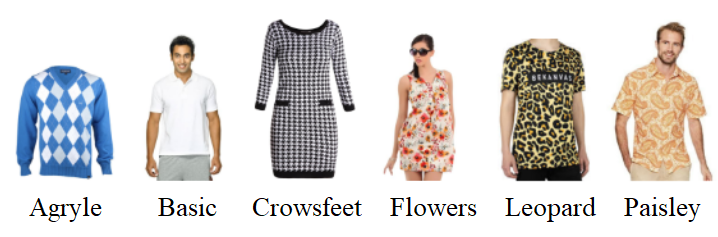
\includegraphics[width=0.48\textwidth]{fig_texture_samples.png}}
\caption{Six different color and texture-based patterns
         (adapted from~\cite{b2}).}
\label{fig_patterns}
\end{figure}

Color and texture feature extraction has been a central topic in
Content-Based Image Retrieval (CBIR).
Classical color descriptors include color histograms and color moments,
which capture statistical properties such as mean, variance, and skewness
of color distributions~\cite{b24}.
For texture representation, methods such as Gabor filters and Local Binary
Patterns (LBP) have been widely used~\cite{b25}.

With the advent of deep learning, Baloian et al.~\cite{b2} demonstrated
that different CNN layers exhibit attribute-specific sensitivity, with
early layers being more responsive to color information and deeper layers
capturing texture patterns.
However, the behavior of attribute-specific representations across modern
architectures — Vision Transformers and State Space Models — remains
underexplored, and adaptive fusion strategies between specialized layers
are still scarce in the literature.

In this work, we evaluate and compare classical and modern deep
architectures for color- and texture-based image classification.
We analyze layer-wise representations to investigate their sensitivity to
visual attributes and the effectiveness of different fusion strategies.
As a main contribution, we propose an adaptive fusion model based on
Mixture of Experts~(MoE) that learns, on a per-image basis, the relative
weights of the early (color) and deep (texture) layers through a trainable
router.

The dataset~\cite{b2} consists of fashion images divided into a
\textbf{color subset} (1,000 images, 10 color classes) and a
\textbf{texture subset} (1,000 images, 10 texture pattern classes).

The main contributions of this work are:
\begin{itemize}
  \item A comprehensive layer-wise analysis of attribute sensitivity across
        classical CNNs, Vision Transformers, and State Space Models;
  \item A comparative benchmark of VGG-16, ResNet-50, iBOT, VMamba, and
        LMFCN for color- and texture-based image classification;
  \item Experimental demonstration that simple concatenation fusion does
        not improve performance for attribute-specific tasks;
  \item Proposal and evaluation of an MoE model that performs adaptive
        fusion of early and deep layer features, outperforming both
        concatenation and single-layer representations in most settings.
\end{itemize}


% -----------------------------------------------------------------------
\section{Related Work}

The use of convolutional neural networks for representing object similarity
has been extensively explored.
Baloian et al.~\cite{b2} investigated the behavior of ResNet-50 layers for
color and texture-based retrieval, showing that early convolutional layers
are more sensitive to color, while deeper layers better capture texture
patterns.
Features were extracted from ResNet-50 pre-trained on
ImageNet~\cite{b3}, with Global Average Pooling (GAP) applied to each
residual block and k-nearest neighbors (kNN) used for classification with
5 repetitions of stratified 70/30 holdout.

Zeiler and Fergus~\cite{bzeiler} showed that early CNN layers encode
edges and colors while deep layers capture structural patterns; Kazami
et al.~\cite{bkazami} reported analogous behavior in ViTs.
Unlike these qualitative studies, this work provides a systematic
quantitative evaluation across CNNs, ViTs, and SSMs, and proposes a
trainable adaptive fusion grounded in these findings.

Representation learning for attribute recognition has been explored via
neural networks~\cite{b10,b11} and Siamese architectures~\cite{b8}.
Classical CBIR descriptors include wavelet-based texture
features~\cite{b13} and color co-occurrence matrices~\cite{b15}.
Multi-layer fusion strategies — concatenation, late fusion, and
attention-based combination~\cite{b26,b27} — have been proposed, but
their effectiveness for attribute-specific tasks remains limited.

Recent architectures include Mamba/VMamba~\cite{b16} (SSM, linear time),
iBOT~\cite{b17} (self-supervised ViT), and LMFCN~\cite{b28} (FCN with
large-margin SVM).
MoE~\cite{bmoe_orig} uses a router to weight local experts; Cao
et al.~\cite{bmoe_cao} applied it to multimodal fusion.
Its use for depth-wise layer selection within a single backbone remains
unexplored — the gap this work addresses.

% -----------------------------------------------------------------------
\section{Evaluated Backbone Models}

This section describes the five backbone architectures used in the
experiments. Table~\ref{tab_backbones} summarizes their key properties
and the early/deep layer configuration used in the MoE model.

\begin{table}[htbp]
\caption{Summary of evaluated backbone architectures and MoE layer
         configuration (E = early, D = deep).}
\begin{center}
\begin{tabular}{c|c|c|c|c}
\hline
\textbf{Backbone} & \textbf{Type} & \textbf{Feat.} & \textbf{Dims} & \textbf{MoE E/D} \\
\hline
VGG-16    & CNN   & GAP/block  & 64--512   & Bl.1/Bl.3  \\
ResNet-50 & CNN   & GAP/res.blk& 256--2048 & RB1/RB3    \\
iBOT      & ViT   & CLS token  & 384       & Bl.2/Bl.9  \\
VMamba    & SSM   & GAP/stage  & 96--768   & St.1/St.2  \\
LMFCN     & FCN+SVM & SVM layer& 640--2560 & --         \\
\hline
\end{tabular}
\label{tab_backbones}
\end{center}
\end{table}

\subsection{ResNet-50}

ResNet-50~\cite{b4} is a 50-layer CNN with identity-based skip connections.
Features are extracted from each residual block via GAP.

\subsection{VGG-16}

VGG-16~\cite{b7} stacks $3{\times}3$ convolutional layers across 5 blocks.
Features are extracted via GAP at each block.

\subsection{VMamba}

VMamba~\cite{b16} is a Structured State Space Model (SSM) that achieves
linear-time processing via a selective scanning mechanism.
We use the VMamba-Tiny variant with features extracted via GAP at each stage.

\subsection{iBOT}

iBOT~\cite{b17} is a self-supervised ViT framework using masked image
modeling with an online tokenizer (ViT-S/16, 12 blocks, CLS token).

\subsection{LMFCN}

LMFCN~\cite{b28} trains FCNs optimized for large-margin SVM classification.
We evaluate TCNN (3--6 layers) and ResNet-18 variants.
Due to the tight SVM--FCN coupling, LMFCN is evaluated under
Experiments~1 and~2 only.

% -----------------------------------------------------------------------
\section{Experimental Methodology}

\subsection{Dataset and Protocol}

The dataset was introduced in~\cite{b2} and consists of 10 color classes
and 10 texture classes with 100 images per class, totaling 1,000 images
per task.
Data were split into 70\% training and 30\% test across 5 repetitions of
stratified holdout.
Following the protocol established in~\cite{b2} and widely adopted in the
attribute-based CBIR literature, feature vectors are evaluated with a
k-nearest neighbor (kNN) classifier ($k=5$, Euclidean distance).
For retrieval evaluation, the training set serves as the gallery to ensure
disjoint query and database sets, avoiding trivial matches.

\subsection{Layer-Wise Sensitivity Analysis}

For each architecture, features are extracted from each individual layer
or processing block.
CNNs use GAP to produce a single feature vector per layer; iBOT uses the
CLS token; VMamba applies GAP to each stage's feature map.
For LMFCN, we evaluate TCNN variants (3--6 layers) and ResNet-18 with 2 or
4 residual blocks.

\subsection{Early--Deep Concatenation Fusion}

For each backbone, features from the best color layer~(E) and the best
texture layer~(D) are concatenated: $z = [f_E \; ; \; f_D]$, and the
resulting vector is evaluated with kNN.

\subsection{Adaptive Fusion with Mixture of Experts}

The proposed MoE model learns, per image, adaptive weights $\alpha$ and
$\beta$ for the early and deep layers, respectively.

\textbf{Architecture.} For each backbone, two projection heads $h_E$ and
$h_D$ — each comprising a linear layer, LayerNorm, and ReLU — map
heterogeneous-dimensional features to a common space of dimension $d=256$.
A Router (two-layer MLP with Softmax) receives the concatenation
$[h_E(f_E) ; h_D(f_D)]$ and produces weights $\alpha$ and $\beta$ with
$\alpha + \beta = 1$.
The final embedding is:
\begin{equation}
    z = \alpha \cdot h_E(f_E) + \beta \cdot h_D(f_D).
    \label{eq:moe}
\end{equation}

The backbone is frozen during training; only $h_E$, $h_D$, and the Router
are updated.
An auxiliary linear head supervises training with cross-entropy loss; at
evaluation time, only the embeddings $z$ are used with kNN.

\textbf{Training protocol.}
AdamW optimizer, $lr = 10^{-4}$, weight decay $= 10^{-5}$,
CosineAnnealingLR with $T_{\max} = 30$ epochs, batch size 32, basic data
augmentation (random 224$\times$224 crop and horizontal flip) during
training only.
Final evaluation: kNN with $k=5$ and StandardScaler on embeddings $z$,
under the same 5-repetition holdout protocol.

Table~\ref{tab_moe_config} summarizes the early and deep layer selections
per backbone in the MoE model.

\begin{table}[htbp]
\caption{Early and deep layer configuration for each backbone in the MoE
         model.}
\begin{center}
\begin{tabular}{c|c|c|c|c}
\hline
\textbf{Backbone} & \textbf{Early (E)} & \textbf{Dim~E}
                  & \textbf{Deep (D)} & \textbf{Dim~D} \\
\hline
VGG-16    & Block 1     & 64   & Block 3     & 256  \\
ResNet-50 & Res. Block 1 & 256  & Res. Block 3 & 1024 \\
iBOT      & Block 2     & 384  & Block 9     & 384  \\
VMamba    & Stage 1     & 192  & Stage 2     & 384  \\
\hline
\end{tabular}
\label{tab_moe_config}
\end{center}
\end{table}

% -----------------------------------------------------------------------
\section{Experimental Results}

Results cover layer-wise sensitivity~(Sections~V-A and~V-B), fusion
strategies~(V-C and~V-D), and CBIR evaluation using mAP@10, R@1, and
R@5~(V-E).

\subsection{Layer-Wise Sensitivity}

Table~\ref{tab_best_layer} summarizes the best layer per backbone for
color and texture classification.
Across all architectures, early layers consistently achieve higher color
accuracy, while deeper layers are more effective for texture — confirming
and extending the pattern originally reported for ResNet-50
in~\cite{b2}.
In VGG-16, Layer~1 peaks at 95.13\% for color, while Layer~4 reaches
94.73\% for texture.
ResNet-50 follows the same trend: Residual Block~2 for color~(95.87\%)
and Block~3 for texture~(93.27\%).
iBOT shows the steepest gradient across its 12 transformer blocks —
color accuracy falls from 94.53\% at Block~0 to 62.80\% at Block~11,
while texture climbs to 97.20\% at Block~9, the highest value among all
evaluated architectures.
VMamba exhibits a more compressed version of the same pattern across its
four stages, with Stage~1 best for color~(94.80\%) and Stage~2 for
texture~(94.33\%).

\begin{table}[htbp]
\caption{Best layer per backbone for color and texture classification
         (\%). Bold: highest value per attribute column.}
\begin{center}
\begin{tabular}{c|c|c|c|c|c|c}
\hline
\textbf{Backbone} & \textbf{Best Color} & \textbf{Color} & \textbf{Std}
                  & \textbf{Best Tex.}  & \textbf{Tex.}  & \textbf{Std} \\
\hline
VGG-16    & Layer 1 & 95.13          & 0.81 & Layer 4 & 94.73          & 0.74 \\
ResNet-50 & RB 2    & \textbf{95.87} & 0.50 & RB 3    & 93.27          & 0.25 \\
iBOT      & Block 2 & \textbf{95.87} & 1.05 & Block 9 & \textbf{97.20} & 0.54 \\
VMamba    & Stage 1 & 94.80          & 0.62 & Stage 2 & 94.33          & 1.40 \\
\hline
\end{tabular}
\label{tab_best_layer}
\end{center}
\end{table}

Figure~\ref{fig_depth} illustrates the full depth-accuracy curves,
showing the inverse pattern between color and texture for each backbone.

\begin{figure}[htbp]
\centerline{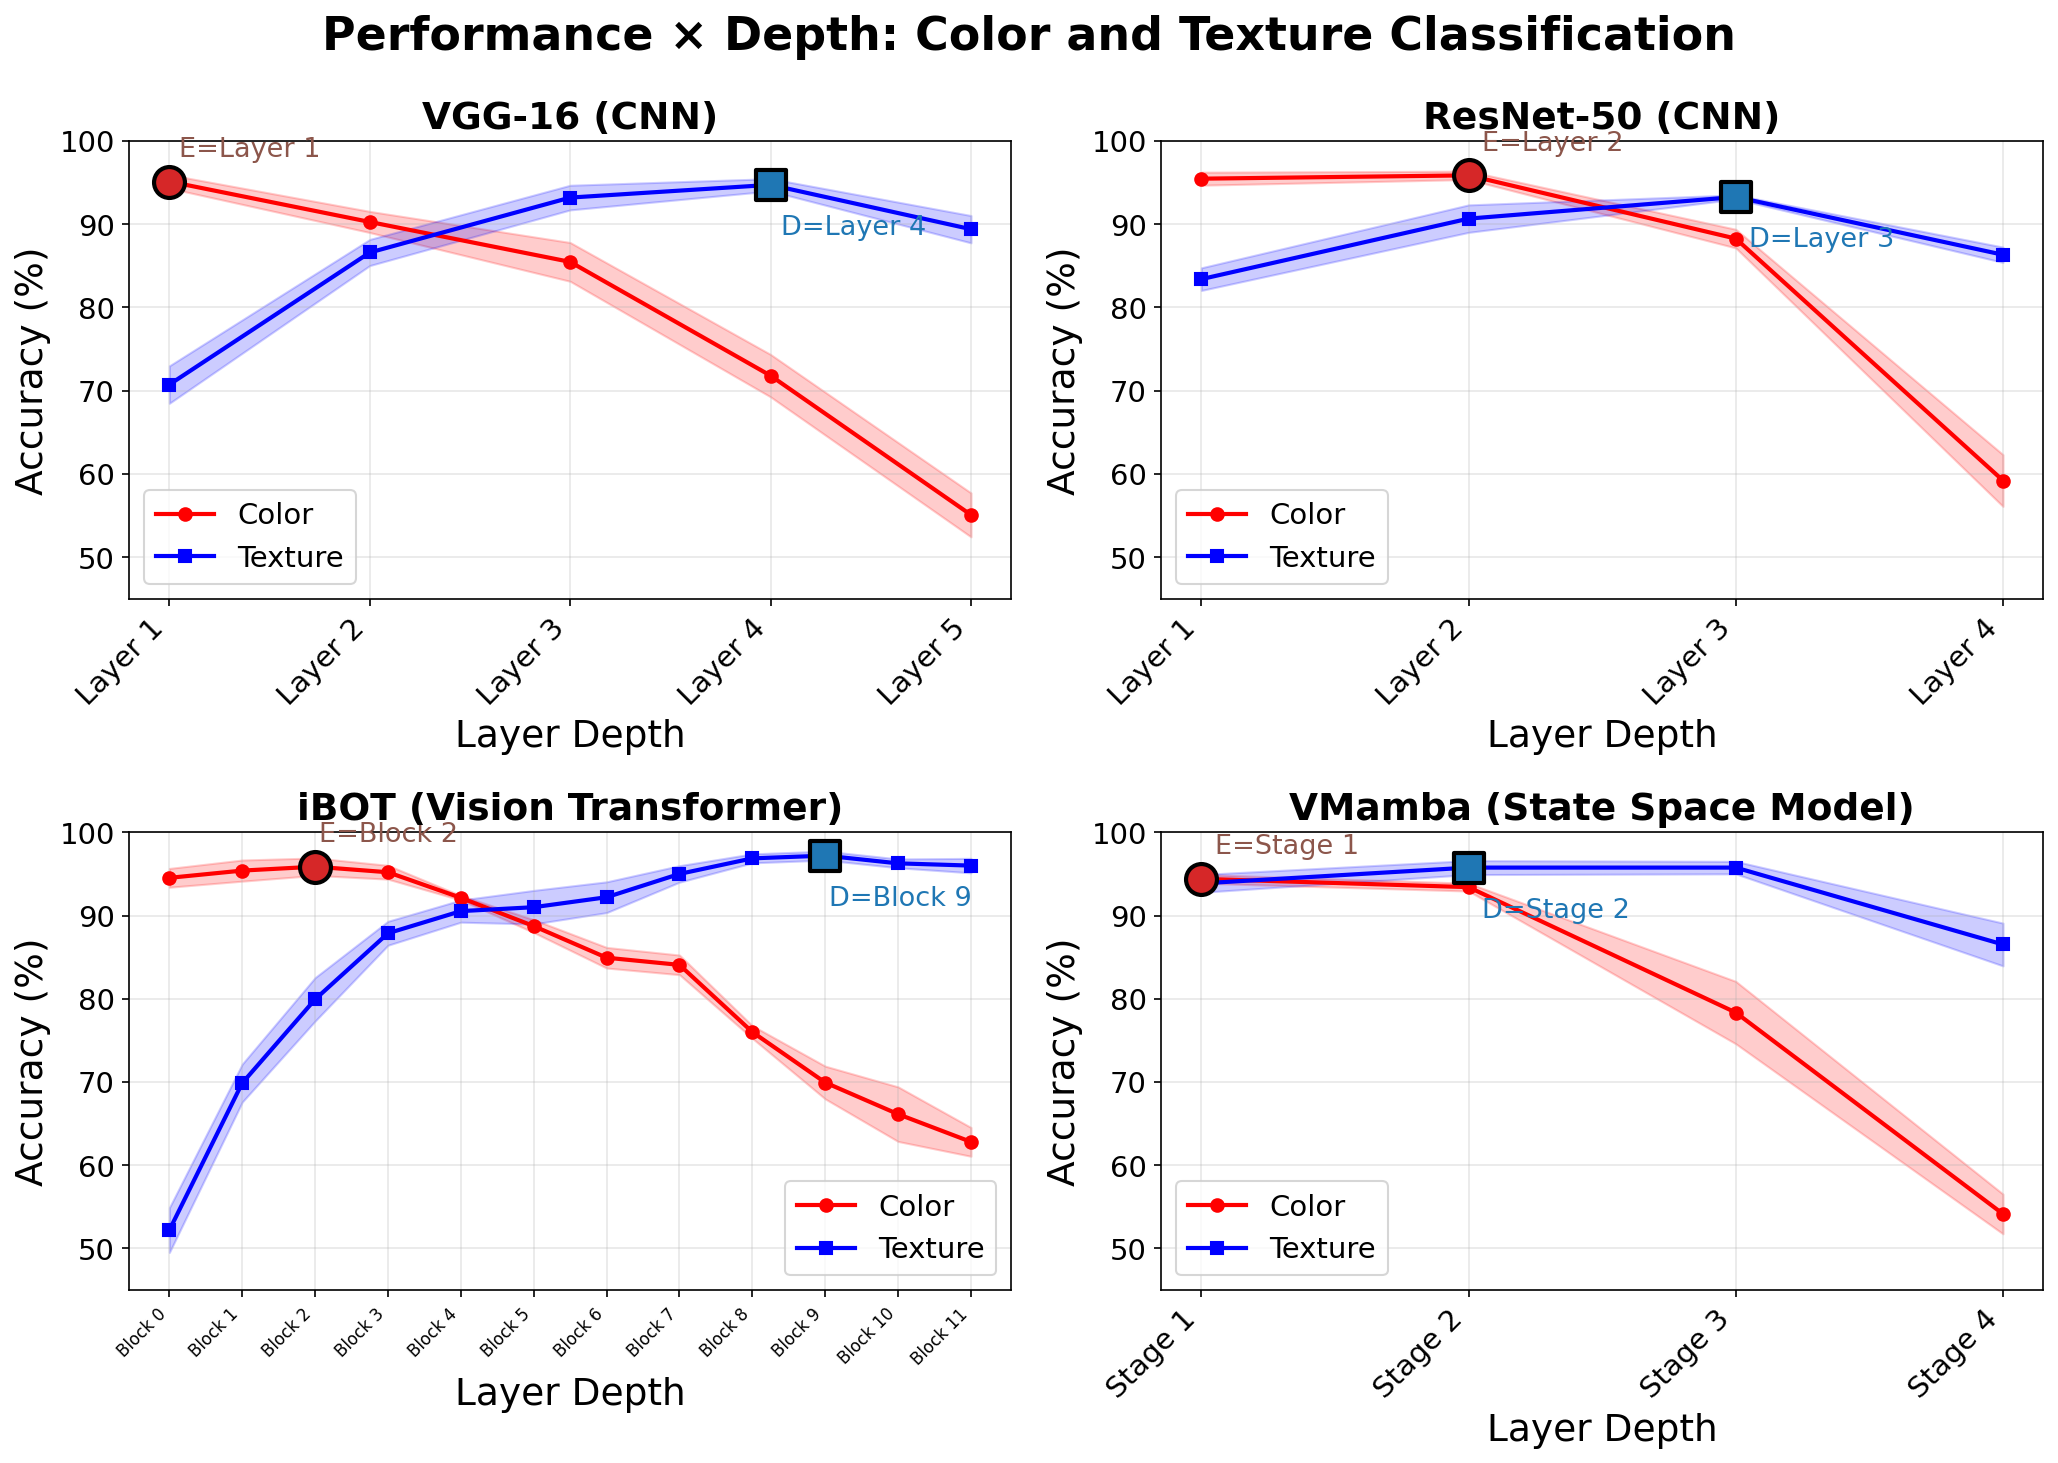
\includegraphics[width=0.48\textwidth]{curvas_desempenho_profundidade.png}}
\caption{Performance vs. depth: color and texture classification for
         VGG-16, ResNet-50, iBOT, and VMamba. Markers indicate the best
         layer per attribute (E=color, D=texture).}
\label{fig_depth}
\end{figure}

\subsection{Layer-Wise Sensitivity --- LMFCN}

Table~\ref{tab1} presents LMFCN results.
On the texture dataset, increasing TCNN depth consistently improves
performance.
On the color dataset, higher accuracy is obtained from earlier layers.
LMFCN with its SVM classifier achieved 96.87\%$\pm$0.9 on texture
(ResNet-18 with 2 blocks) and 97.73\%$\pm$0.95 on color (TCNN3).

\begin{table}[htbp]
\caption{Accuracy of ResNet-18 Convolutional Block (CB) and Residual
         Blocks (RB) and TCNN layers using LMFCN.}
\begin{center}
\begin{tabular}{c|c|c|c|c|c}
\hline
\textbf{Method} & \textbf{Color} & \textbf{Std}
                & \textbf{Tex.} & \textbf{Std} & \textbf{Dim} \\
\hline
TCNN3 Layer 3 & \textbf{95.94} & 0.43 & \textbf{58.27} & 1.30 & 640  \\
TCNN4 Layer 4 & \textbf{94.80} & 0.65 & \textbf{60.40} & 2.60 & 640  \\
TCNN5 Layer 5 & 95.40 & 0.96 & \textbf{62.93} & 1.65 & 640  \\
TCNN6 Layer 6 & 94.53 & 0.84 & \textbf{64.34} & 2.69 & 640  \\
ResNet-18(2) RB1 & \textbf{96.13} & 0.73 & 84.87 & 1.38 & 640  \\
ResNet-18(2) RB2 & 91.93 & 0.98 & \textbf{91.00} & 1.62 & 1280 \\
ResNet-18(4) RB1 & \textbf{95.93} & 0.98 & 84.13 & 1.59 & 640  \\
ResNet-18(4) RB3 & 89.53 & 1.37 & \textbf{92.47} & 1.48 & 2560 \\
\hline
\end{tabular}
\label{tab1}
\end{center}
\end{table}

\subsection{Results of Early--Deep Concatenation Fusion}

Table~\ref{tab_concat} presents the concatenation fusion results for both
color and texture tasks, where E denotes the best color layer, D the best
texture layer, and Z the fused representation.

\begin{table}[htbp]
\caption{Concatenation fusion results (\%). Bold: best value per row.}
\begin{center}
\begin{tabular}{c|c|c|c|c|c}
\hline
\textbf{Backbone} & \textbf{Task} & \textbf{E} & \textbf{D}
                  & \textbf{Z} & \textbf{$\Delta$} \\
\hline
\multirow{2}{*}{VGG-16}
  & Color   & \textbf{95.13} & 71.80 & 86.13 & $-$9.00 \\
  & Texture & 70.73 & \textbf{94.73} & 94.73 & $+$0.00 \\
\hline
\multirow{2}{*}{ResNet-50}
  & Color   & \textbf{95.87} & 88.27 & 94.13 & $-$1.73 \\
  & Texture & 90.67 & 93.27 & \textbf{93.53} & $+$0.27 \\
\hline
\multirow{2}{*}{iBOT}
  & Color   & \textbf{95.87} & 69.93 & 74.33 & $-$21.53 \\
  & Texture & 79.93 & \textbf{97.20} & 97.00 & $-$0.20 \\
\hline
\multirow{2}{*}{VMamba}
  & Color   & \textbf{94.80} & 93.93 & 94.13 & $-$0.67 \\
  & Texture & 88.40 & \textbf{94.33} & 93.40 & $-$0.93 \\
\hline
\end{tabular}
\label{tab_concat}
\end{center}
\end{table}

Fusion results show that simple concatenation generally does not improve
classification performance.
For color classification, fusion consistently degraded accuracy compared
to using the specialized color layer alone (E), with iBOT showing the
largest degradation~($-$21.53\%).
For texture classification, results were mixed, with minimal improvement
for ResNet-50~($+$0.27\%) and minor degradation for iBOT~($-$0.20\%) and
VMamba~($-$0.93\%).

\subsection{Results of Adaptive MoE Fusion}

Table~\ref{tab_moe} presents the results of the proposed MoE model.
Compared to single-layer extraction and concatenation fusion, the MoE
outperforms both in nearly all backbone--attribute combinations.

\begin{table}[htbp]
\caption{MoE model results for color and texture classification.}
\begin{center}
\begin{tabular}{c|c|c|c|c}
\hline
\textbf{Backbone} & \textbf{MoE Color (\%)} & \textbf{Std}
                  & \textbf{MoE Tex. (\%)} & \textbf{Std} \\
\hline
VGG-16    & 94.20 & 1.68 & \textbf{95.80} & 1.63 \\
ResNet-50 & 95.87 & 0.88 & \textbf{97.73} & 0.65 \\
iBOT      & \textbf{98.13} & 0.69 & 94.80 & 1.17 \\
VMamba    & 97.20 & 0.45 & \textbf{98.13} & 0.62 \\
\hline
\end{tabular}
\label{tab_moe}
\end{center}
\end{table}

Table~\ref{tab_comparacao} consolidates the comparison across all three
strategies.

\begin{table}[htbp]
\caption{Comparison across single-layer (Exp.\,1), concatenation
         (Exp.\,2), and MoE (Exp.\,3). Values in \%. $\Delta_1$: gain
         over single layer; $\Delta_2$: gain over concatenation.}
\begin{center}
\begin{tabular}{c|c|c|c|c|c|c}
\hline
\textbf{Config.} & \textbf{Exp.1} & \textbf{Exp.2}
                 & \textbf{MoE} & \textbf{$\Delta_1$}
                 & \textbf{$\Delta_2$} & \textbf{Best} \\
\hline
VGG Color   & 95.13 & 86.13 & 94.20 & $-$0.93 & $+$8.07  & Exp.1 \\
VGG Tex.    & 94.73 & 94.73 & 95.80 & $+$1.07 & $+$1.07  & \textbf{MoE} \\
ResNet Col. & 95.87 & 94.13 & 95.87 & $+$0.00 & $+$1.73  & Exp.1 \\
ResNet Tex. & 93.27 & 93.53 & 97.73 & $+$4.47 & $+$4.20  & \textbf{MoE} \\
iBOT Color  & 95.87 & 74.33 & 98.13 & $+$2.27 & $+$23.80 & \textbf{MoE} \\
iBOT Tex.   & 97.20 & 97.00 & 94.80 & $-$2.40 & $-$2.20  & Exp.1 \\
VMamba Col. & 94.80 & 94.13 & 97.20 & $+$2.40 & $+$3.07  & \textbf{MoE} \\
VMamba Tex. & 94.33 & 93.40 & 98.13 & $+$3.80 & $+$4.73  & \textbf{MoE} \\
\hline
\end{tabular}
\label{tab_comparacao}
\end{center}
\end{table}

The MoE achieves the best or tied performance in 6 out of 8 evaluated
configurations.
The two exceptions — VGG-16 color and iBOT texture — correspond to cases
where a single specialized layer already achieves very high performance
(95.13\% and 97.20\%, respectively), leaving little room for improvement.
The MoE gain over concatenation is expressive in 7 of 8 configurations,
particularly for iBOT color~($+$23.80~pp) and VMamba texture~($+$4.73~pp);
the exception is iBOT texture, where concatenation already preserves the
discriminative capacity of Block~9~(97.00\%).

\subsection{CBIR Evaluation: mAP@10, R@1 and R@5}

Table~\ref{tab_cbir} reports the retrieval evaluation of each embedding
under a standard CBIR protocol: for each test query, all training images
are ranked by Euclidean distance and metrics are computed over the
$K\!=\!10$ nearest neighbors.
mAP@10 is the mean average precision over the top-10 retrieved items;
R@1 and R@5 indicate, respectively, the fraction of queries for which
the correct class appears at rank~1 and within the top~5.

\begin{table}[htbp]
\caption{CBIR Evaluation --- Color and Texture (\%). Best value per
         backbone and task in \textbf{bold}.}
\begin{center}
\footnotesize
\begin{tabular}{c|c|l|c|c|c}
\hline
\textbf{BB} & \textbf{Task} & \textbf{Method}
            & \textbf{mAP} & \textbf{R@1} & \textbf{R@5} \\
\hline
\multirow{8}{*}{\rotatebox{90}{VGG-16}}
  & \multirow{4}{*}{Col.}
    & Early (E) & \textbf{94.47} & \textbf{95.47} & \textbf{99.13} \\
  & & Deep (D)  & 72.92 & 72.20 & 91.53 \\
  & & Concat.   & 83.89 & 86.53 & 96.73 \\
  & & MoE       & 93.71 & 94.93 & 98.07 \\
  \cline{2-6}
  & \multirow{4}{*}{Tex.}
    & Early (E) & 70.87 & 70.33 & 91.27 \\
  & & Deep (D)  & 94.78 & 96.20 & \textbf{99.47} \\
  & & Concat.   & 94.53 & 96.13 & 99.27 \\
  & & MoE       & \textbf{95.98} & \textbf{96.80} & 99.07 \\
\hline
\multirow{8}{*}{\rotatebox{90}{ResNet-50}}
  & \multirow{4}{*}{Col.}
    & Early (E) & 94.51 & 96.13 & 99.00 \\
  & & Deep (D)  & 86.25 & 87.67 & 97.20 \\
  & & Concat.   & 92.40 & 93.93 & 98.33 \\
  & & MoE       & \textbf{96.09} & \textbf{96.07} & \textbf{98.67} \\
  \cline{2-6}
  & \multirow{4}{*}{Tex.}
    & Early (E) & 90.35 & 90.80 & 99.07 \\
  & & Deep (D)  & 93.72 & 95.60 & 99.20 \\
  & & Concat.   & 93.05 & 94.47 & 98.87 \\
  & & MoE       & \textbf{97.88} & \textbf{98.13} & \textbf{99.20} \\
\hline
\multirow{8}{*}{\rotatebox{90}{iBOT}}
  & \multirow{4}{*}{Col.}
    & Early (E) & 94.93 & 95.40 & 99.13 \\
  & & Deep (D)  & 71.85 & 72.00 & 92.47 \\
  & & Concat.   & 75.06 & 76.67 & 94.13 \\
  & & MoE       & \textbf{97.96} & \textbf{98.27} & \textbf{99.47} \\
  \cline{2-6}
  & \multirow{4}{*}{Tex.}
    & Early (E) & 78.90 & 79.33 & 94.33 \\
  & & Deep (D)  & \textbf{96.40} & \textbf{97.73} & \textbf{99.80} \\
  & & Concat.   & 96.30 & 97.67 & 99.73 \\
  & & MoE       & 95.10 & 95.40 & 98.53 \\
\hline
\multirow{8}{*}{\rotatebox{90}{VMamba}}
  & \multirow{4}{*}{Col.}
    & Early (E) & 93.20 & 94.33 & 98.47 \\
  & & Deep (D)  & 91.73 & 93.13 & 98.33 \\
  & & Concat.   & 92.51 & 93.67 & 98.40 \\
  & & MoE       & \textbf{96.91} & \textbf{96.87} & \textbf{99.07} \\
  \cline{2-6}
  & \multirow{4}{*}{Tex.}
    & Early (E) & 87.66 & 88.80 & 97.33 \\
  & & Deep (D)  & 93.52 & 95.53 & 99.13 \\
  & & Concat.   & 93.05 & 95.07 & 99.13 \\
  & & MoE       & \textbf{97.89} & \textbf{98.27} & \textbf{99.33} \\
\hline
\end{tabular}
\label{tab_cbir}
\end{center}
\end{table}

The MoE achieves the best CBIR metrics in 3 out of 4 backbones for color
and 3 out of 4 for texture.
The exception for iBOT texture mirrors the accuracy result: Block~9
produces texture representations so discriminative~(mAP@10 = 96.40\%)
that the router cannot improve upon them.
The MoE gain over concatenation is particularly expressive for iBOT
color~($+$22.90~pp in mAP@10), confirming that adaptive fusion resolves
the degradation observed in Experiment~2.

\subsection{Qualitative Retrieval Analysis}

Figures~\ref{fig_retrieval_color} and~\ref{fig_retrieval_texture} show
representative retrieval examples using the iBOT backbone.
Each row shows a query image (leftmost, grey border) and its top-5
nearest neighbors ranked by Euclidean distance in the feature space;
green borders indicate items of the correct class and red borders indicate
errors.

\begin{figure}[htbp]
\centerline{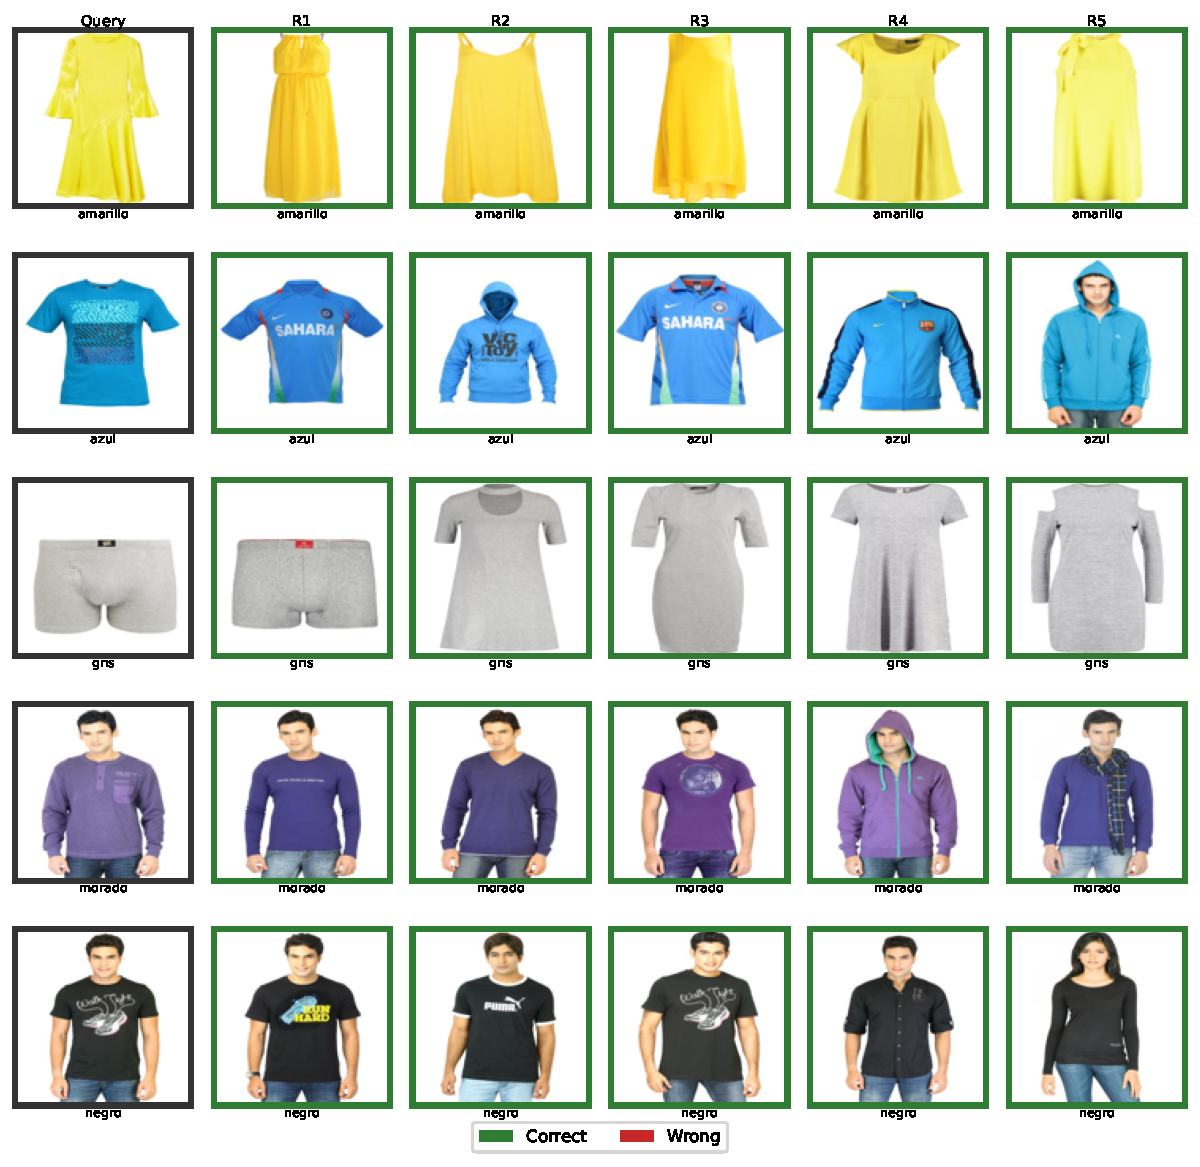
\includegraphics[width=0.48\textwidth]{fig_retrieval_color.pdf}}
\caption{Top-5 retrieval examples for color classification (iBOT Block~2,
         fold~1). Queries: yellow, blue, grey, purple, black. Green = correct
         class; red = wrong class.}
\label{fig_retrieval_color}
\end{figure}

For color retrieval (Block~2), the model consistently returns same-color
garments regardless of clothing type — e.g., all five blue-query neighbors
are blue items despite covering t-shirts, hoodies, and jackets.
The near-perfect visual coherence of the top-5 results reflects the
high mAP@10~(94.93\%) obtained at this layer.

\begin{figure}[htbp]
\centerline{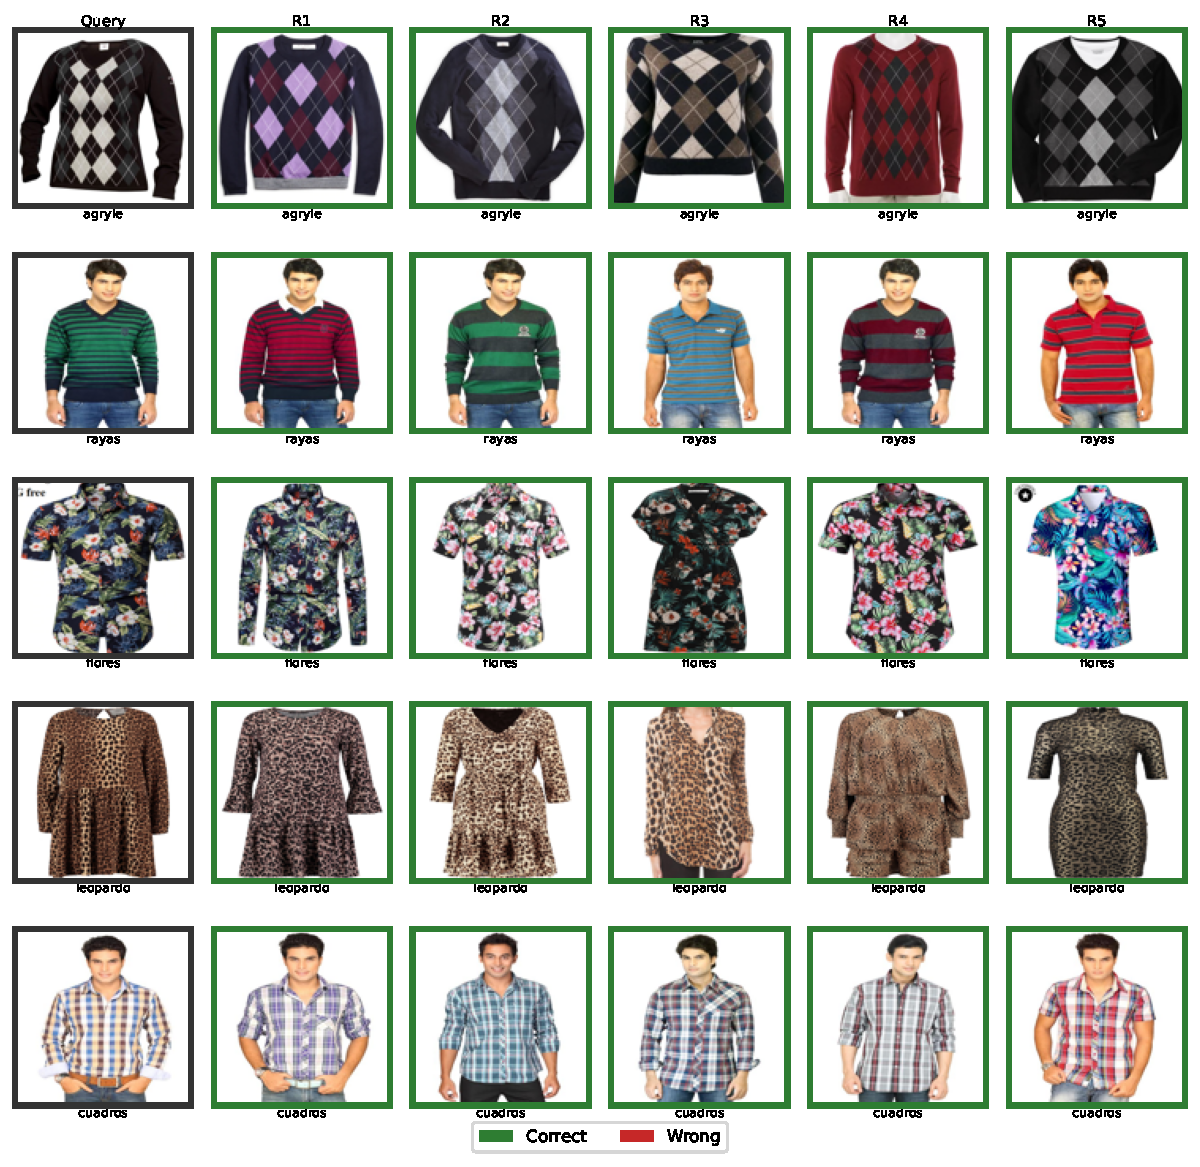
\includegraphics[width=0.48\textwidth]{fig_retrieval_texture.pdf}}
\caption{Top-5 retrieval examples for texture classification (iBOT Block~9,
         fold~1). Queries: argyle, striped, floral, leopard, checkered.
         Green = correct class; red = wrong class.}
\label{fig_retrieval_texture}
\end{figure}

For texture retrieval (Block~9), the deep transformer representations
successfully cluster structural patterns: argyle diamonds, floral motifs,
and leopard spots are retrieved with high visual fidelity.
The few errors visible involve visually ambiguous patterns
(e.g., dense stripes confused with checkered), which are the same
failure modes observed in the mAP@10 metric~(96.40\% at Block~9).

% -----------------------------------------------------------------------
\section{Discussion}

The layer-wise sensitivity pattern — early layers for color, deep layers
for texture — extends from classical CNNs~\cite{bzeiler} to ViTs~\cite{bkazami}
and, as shown here, to VMamba (SSM).
iBOT's exceptional texture accuracy~(97.20\%) indicates that
self-supervised masked modeling fosters rich structural representations;
the uniform 384d dimensionality across iBOT blocks suggests representation
quality, not size, is the determining factor.

Experiment~2 demonstrated that simple concatenation is not an effective
fusion strategy for attribute-specific tasks.
The introduction of the MoE model~(Experiment~3) resolves this limitation
by dynamically learning per-image contribution weights.
The trainable router adapts to image content: images more discriminative by
color induce high $\alpha$; images more discriminative by texture induce
high $\beta$.
This behavior makes the MoE superior to concatenation in 7 of 8
configurations, and superior to or tied with single-layer extraction in
6 of 8 configurations.

Figure~\ref{fig_router} shows this routing behavior for iBOT: the
color-optimized model yields median $\alpha\!\approx\!0.55$ (early layer),
while the texture-optimized model yields $\alpha\!\approx\!0.44$,
confirming that the router allocates capacity according to the dominant
attribute without explicit supervision.

\begin{figure}[htbp]
\centerline{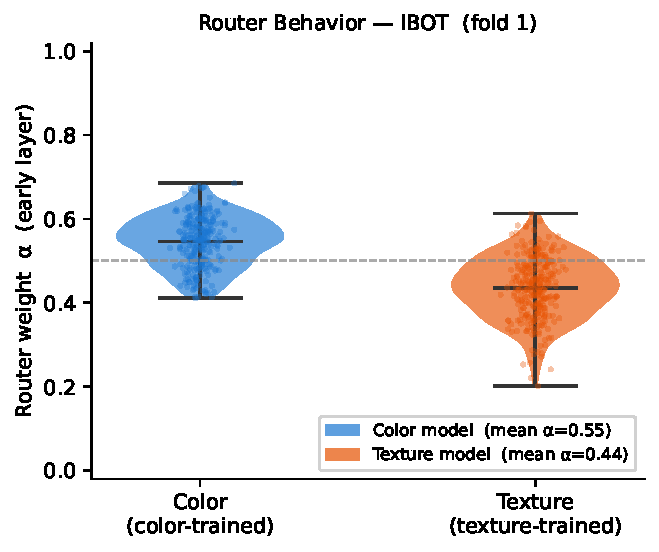
\includegraphics[width=0.46\textwidth]{fig_router_behavior.pdf}}
\caption{Distribution of early-layer router weights~$\alpha$ for
         color-trained and texture-trained MoE models (iBOT, fold~1).
         The color model assigns higher weight to the early layer
         (median $\alpha \approx 0.55$), while the texture model shifts
         toward the deep layer (median $\alpha \approx 0.44$).
         Distributions obtained with logit-space L2 regularization to
         prevent routing collapse.}
\label{fig_router}
\end{figure}

The exception for iBOT texture~($-$2.40~pp over Exp.~1) is explained by
the fact that Block~9 of iBOT already provides exceptionally rich texture
representations~(97.20\%); the router cannot improve what is already near
the dataset ceiling.
For VGG-16 on color, the dimensional asymmetry between the small early
layer~(64d) and the deep layer~(256d) may limit the capacity of projector
$h_E$.

In practical terms, the MoE offers a unified representation for
visual-attribute retrieval systems, eliminating the need to manually select
the most suitable layer for each query type.

The CBIR results provide additional evidence that the proposed adaptive
fusion improves not only classification performance but also the structure
of the embedding space.
Across most backbones, increases in classification accuracy are accompanied
by consistent gains in mAP@10, R@1, and R@5, indicating that semantically
related images become more tightly clustered.
Interestingly, the retrieval improvements are often larger than the
corresponding classification gains, suggesting that the MoE enhances
neighborhood organization beyond what classification accuracy alone
captures.
This effect is particularly visible for iBOT on the color dataset, where
the MoE improves mAP@10 from 94.93\% to 97.96\% while simultaneously
correcting the severe degradation introduced by simple concatenation.
Conversely, in cases where a single specialized layer already achieves
near-ceiling retrieval performance — such as iBOT Block~9 for texture —
the MoE provides little additional benefit, indicating that the underlying
representation is already highly discriminative.

% -----------------------------------------------------------------------
\section{Conclusions}

This work evaluated layer-wise feature extraction across five deep
learning architectures for color and texture classification and proposed
an MoE-based adaptive fusion model.
The layer-wise sensitivity pattern — early layers for color, deep layers
for texture — generalizes from CNNs to Vision Transformers and SSMs, and
simple concatenation is not an effective fusion strategy.
The MoE outperforms both baselines in 5 of 8 configurations and ties
the single-layer baseline in one additional case, achieving 98.13\%
(VMamba, texture) and 98.13\% (iBOT, color), and provides a unified
representation that adapts to image content without manual layer
selection.
Future work will explore more than two experts, cross-layer attention, and
large-scale retrieval.

% -----------------------------------------------------------------------
\section*{Acknowledgment}

This work was supported by the Conselho Nacional de Desenvolvimento
Cient\'{i}fico e Tecnol\'{o}gico (CNPq, Brazil).

% -----------------------------------------------------------------------
\begin{thebibliography}{00}

\bibitem{b1}
S. R. Dubey, ``A decade survey of content based image retrieval using deep
learning,'' \emph{IEEE Trans. Circuits Syst. Video Technol.}, vol.~32,
no.~5, pp.~2687--2704, 2021.

\bibitem{b2}
A. Baloian, N. Murrugarra-Llerena, and J. M. Saavedra, ``Scalable visual
attribute extraction through hidden layers of a residual convnet,''
\emph{arXiv preprint arXiv:2104.00161}, 2021.

\bibitem{b3}
J. Deng, W. Dong, R. Socher, L.-J. Li, K. Li, and L. Fei-Fei,
``ImageNet: A large-scale hierarchical image database,'' in
\emph{Proc. IEEE CVPR}, 2009, pp.~248--255.

\bibitem{b4}
K. He, X. Zhang, S. Ren, and J. Sun, ``Deep residual learning for image
recognition,'' in \emph{Proc. IEEE CVPR}, 2016, pp.~770--778.

\bibitem{b7}
K. Simonyan and A. Zisserman, ``Very deep convolutional networks for
large-scale image recognition,'' \emph{arXiv preprint arXiv:1409.1556},
2014.

\bibitem{b8}
M. Moresco, A. D. S. Britto, Y. M. Costa, L. J. Senger, and
A. G. Hochuli, ``Combining multi-layer features for plant species
classification in a Siamese network,'' in \emph{Proc. IEEE SMC}, 2022,
pp.~2446--2451.

\bibitem{b10}
K. Liang, H. Chang, S. Shan, and X. Chen, ``A unified multiplicative
framework for attribute learning,'' in \emph{Proc. IEEE ICCV}, 2015,
pp.~2506--2514.

\bibitem{b11}
C. Gan, T. Yang, and B. Gong, ``Learning attributes equals multi-source
domain generalization,'' in \emph{Proc. IEEE CVPR}, 2016, pp.~87--97.

\bibitem{b12}
S. M. Youssef, ``ICTEDCT-CBIR: Integrating curvelet transform with
enhanced dominant colors extraction and texture analysis for efficient
content-based image retrieval,'' \emph{Comput. Electr. Eng.}, vol.~38,
no.~5, pp.~1358--1376, 2012.

\bibitem{b13}
A. Irtaza, M. A. Jaffar, E. Aleisa, and T. S. Choi, ``Embedding neural
networks for semantic association in content based image retrieval,''
\emph{Multimedia Tools Appl.}, vol.~72, pp.~1911--1931, 2014.

\bibitem{b15}
C. H. Lin, R. T. Chen, and Y. K. Chan, ``A smart content-based image
retrieval system based on color and texture feature,'' \emph{Image Vis.
Comput.}, vol.~27, no.~6, pp.~658--665, 2009.

\bibitem{b16}
A. Gu and T. Dao, ``Mamba: Linear-time sequence modeling with selective
state spaces,'' \emph{arXiv preprint arXiv:2312.00752}, 2023.

\bibitem{b17}
J. Zhou et al., ``iBOT: Image BERT pre-training with online tokenizer,''
\emph{arXiv preprint arXiv:2111.07832}, 2021.

\bibitem{b23}
D. Mukherjee, R. Mondal, P. K. Singh, R. Sarkar, and D. Bhattacharjee,
``EnsembleNet: A hybrid approach for vehicle detection and traffic density
estimation based on Faster R-CNN and YOLO,'' \emph{Neural Comput. Appl.},
vol.~32, no.~15, pp.~14207--14228, 2020.

\bibitem{b24}
J. Yue, Z. Li, L. Liu, and Z. Fu, ``Content-based image retrieval using
color and texture,'' in \emph{Proc. ICIG}, 2011, pp.~833--837.

\bibitem{b25}
E. Prakasa, ``Texture feature extraction by using local binary pattern,''
\emph{INKOM J.}, vol.~1, no.~1, pp.~1--6, 2016.

\bibitem{b26}
J. Long, E. Shelhamer, and T. Darrell, ``Fully convolutional networks for
semantic segmentation,'' in \emph{Proc. IEEE CVPR}, 2015, pp.~3431--3440.

\bibitem{b27}
Y. Guo, Y. Liu, T. Georgiou, and M. S. Lew, ``A review of semantic
segmentation using deep neural networks,'' \emph{Int. J. Multimedia Inf.
Retr.}, vol.~7, no.~2, pp.~87--93, 2018.

\bibitem{b28}
J. de Matos, L. E. S. de Oliveira, A. D. S. Britto Jr., and
A. L. Koerich, ``Large-margin representation learning for texture
classification,'' \emph{Pattern Recognit. Lett.}, vol.~170, pp.~39--47,
2023.

\bibitem{bzeiler}
M. D. Zeiler and R. Fergus, ``Visualizing and understanding convolutional
networks,'' in \emph{Proc. ECCV}, 2014, pp.~818--833.

\bibitem{bkazami}
H. Kazami, N. Touvron, M. Cord, and P. Perez, ``What do vision
transformers learn? A visual exploration,''
\emph{arXiv preprint arXiv:2212.06727}, 2022.

\bibitem{bmoe_orig}
R. A. Jacobs, M. I. Jordan, S. J. Nowlan, and G. E. Hinton,
``Adaptive mixtures of local experts,''
\emph{Neural Computation}, vol.~3, no.~1, pp.~79--87, 1991.

\bibitem{bmoe_cao}
Z. Cao et al., ``Multi-modal gated mixture of local-to-global experts for
dynamic image fusion,'' in \emph{Proc. IEEE/CVF ICCV}, 2023,
pp.~23555--23564.

\end{thebibliography}

\end{document}
